The goal was to estimate real-time joint kinematic and muscle activation using a moving horizon estimation (MHE). The example is given for a shoulder elevation motion using a 4-DoFs arm actuated by 19 Hill-type muscles. To use MHE, the OCP was split into a succession of smaller one. Each objective function was written as:

\[
\resizebox{0.9\columnwidth}{!}{$
\begin{aligned} \noindent \mathcal{J} = \sum_{n}^{n + n_{mhe}}\underbrace{\omega_1´(\|q_{ref} - q_{est}\|^{2})}_{TRACK\_STATE} ~ + ~ \underbrace{\omega_2\int_t^{t+t_{mhe}} \sum_{i=1}^{8}~Q_{i}^2~dt}_{MINIMIZE\_ STATE} ~ + ~ \underbrace{\omega_3\int_t^{t+t_{mhe}} \sum_{i=1}^{19}~U_{i}^2~dt}_{MINIMIZE\_ ACTIVATION} 
\end{aligned}
$} \addtag \label{eq:ocp_exMHE} 
\]

\noindent where $\omega_1$ =1e4 , $\omega_2$ = 10, $\omega_3$ = 100, $n_{mhe}$ is the number of OCP shooting node and $t_{mhe}$ is OCP duration. $q_{ref}$, $q_{est}$, $Q_i$ and $U_i$ are respectively reference and estimate joints angles, states and muscles activations. \\  
The first term of the objective function (Eq.~\ref{eq:ocp_exMHE}) corresponds to tracking experimental joint angles. Second and third were added for states and muscle controls regularization. Thanks to the high similarity between successive problems, a warm-start strategy using previous solutions was implemented.  
 
 
The shoulder elevation movement was generated with co-activation on two antagonists' muscles groups (triceps, biceps). It lasted for 8s and was discretized using 800 shooting nodes. A windows size of 7 nodes which allows the estimator to run around 50Hz, four times faster than standard biofeedback (13Hz), was chosen. Whereas reference data were generated at 100Hz, only one in two frames was sent to the estimator to correspond with experimental conditions.
 
The estimator was able to forecast the movement kinematic (Fig.~\ref{fig:angulare_angle_MHE}) with a consistent dynamic (Fig.~\ref{fig:muscles_excitations_MHE}). Due to cocontraction, the estimated muscles activations are lower than reference motion activations but with similar pattern. 

\begin{figure*}[t!]
\centering
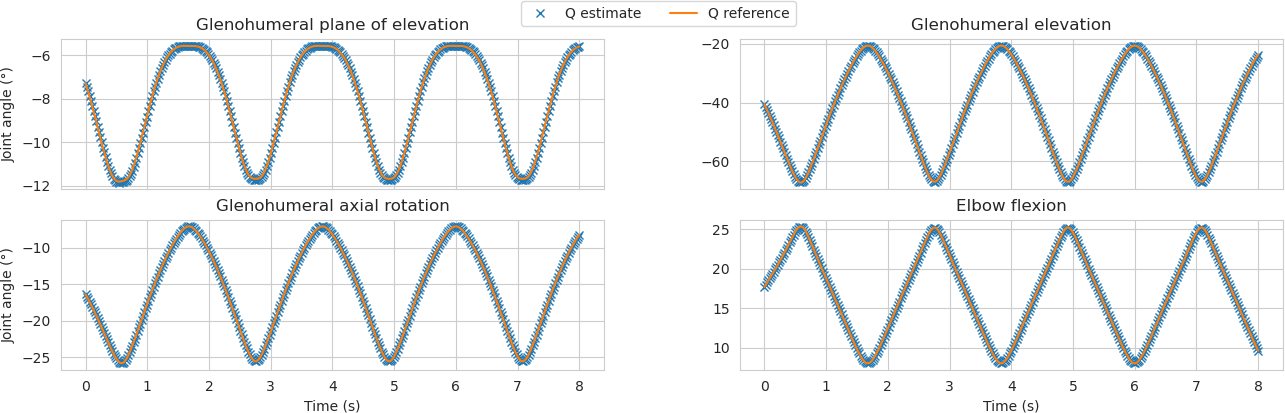
\includegraphics[width=\textwidth]{figures/Articular_angle_MHE.png}\\
\caption{Representation of estimate articlation angles (blue cross) and reference articulation angles (orange line).}
\label{fig:angulare_angle_MHE}
\end{figure*}
\begin{figure*}[t!]
\centering
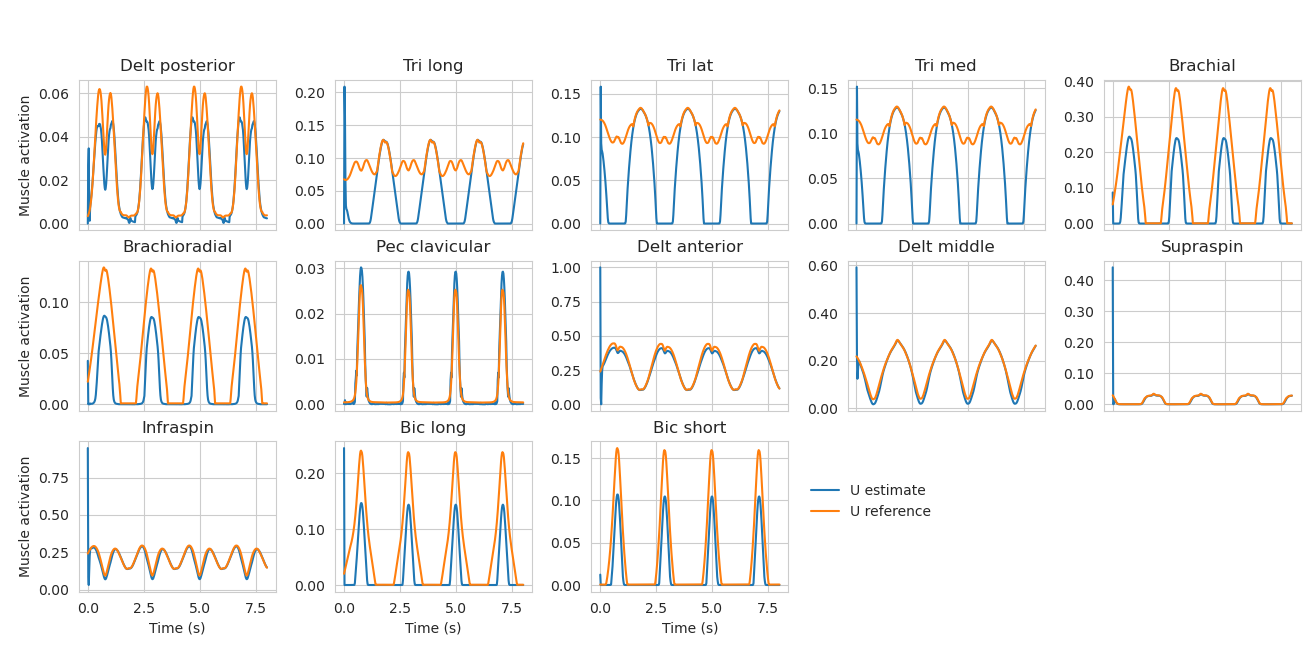
\includegraphics[width=\textwidth]{figures/Muscles_excitations_MHE.png}\\
\caption{Representation of estimate muscles activations (blue) and co-contracted muscles activations (orange) with significative action on motion (activation $>$ 1e-3).}
\label{fig:muscles_excitations_MHE}
\end{figure*}
